\documentclass{beamer}
\usepackage[utf8]{inputenc}

\usetheme{Madrid}
\usecolortheme{default}
\usepackage{amsmath,amssymb,amsfonts,amsthm}
\usepackage{mathtools}
\usepackage{txfonts}
\usepackage{tkz-euclide}
\usepackage{listings}
\usepackage{adjustbox}
\usepackage{array}
\usepackage{gensymb}
\usepackage{tabularx}
\usepackage{gvv}
\usepackage{lmodern}
\usepackage{circuitikz}
\usepackage{tikz}
\lstset{literate={·}{{$\cdot$}}1 {λ}{{$\lambda$}}1 {→}{{$\to$}}1}
\usepackage{graphicx}

\setbeamertemplate{page number in head/foot}[totalframenumber]

\usepackage{tcolorbox}
\tcbuselibrary{minted,breakable,xparse,skins}



\definecolor{bg}{gray}{0.95}
\DeclareTCBListing{mintedbox}{O{}m!O{}}{%
  breakable=true,
  listing engine=minted,
  listing only,
  minted language=#2,
  minted style=default,
  minted options={%
    linenos,
    gobble=0,
    breaklines=true,
    breakafter=,,
    fontsize=\small,
    numbersep=8pt,
    #1},
  boxsep=0pt,
  left skip=0pt,
  right skip=0pt,
  left=25pt,
  right=0pt,
  top=3pt,
  bottom=3pt,
  arc=5pt,
  leftrule=0pt,
  rightrule=0pt,
  bottomrule=2pt,
  toprule=2pt,
  colback=bg,
  colframe=orange!70,
  enhanced,
  overlay={%
    \begin{tcbclipinterior}
    \fill[orange!20!white] (frame.south west) rectangle ([xshift=20pt]frame.north west);
    \end{tcbclipinterior}},
  #3,
}
\lstset{
    language=C,
    basicstyle=\ttfamily\small,
    keywordstyle=\color{blue},
    stringstyle=\color{orange},
    commentstyle=\color{green!60!black},
    numbers=left,
    numberstyle=\tiny\color{gray},
    breaklines=true,
    showstringspaces=false,
}
%------------------------------------------------------------
%This block of code defines the information to appear in the
%Title page
\title %optional
{5.2.30}
\date{17 September, 2025}
%\subtitle{A short story}

\author % (optional)
{INDHIRESH S - EE25BTECH11027}

\begin{document}

\frame{\titlepage}

\begin{frame}{Question}
 Solve the following system of linear equations.
\begin{align*}
    7x - 15y = 2\\
    x + 2y = 3
\end{align*}
\end{frame}

\begin{frame}[allowframebreaks] 
\frametitle{Equation}
    \centering
    \label{tab:parameters}
The given equation can be written as:
\begin{align}
   \myvec{7&-15\\1&2}\Vec{x}=\myvec{2\\3}
   \end{align}
\end{frame}

\begin{frame}
\frametitle{Theoretical Solution}
\begin{align}
   \augvec{2}{1}{7&-15&2\\1&2&3}\xleftrightarrow{R_2\longleftarrow R_2-\frac{1}{7}R_1}\augvec{2}{1}{7&-15&2\\0&\frac{29}{7}&\frac{19}{7}}
\end{align}

\begin{align}
   \augvec{2}{1}{7&-15&2\\0&\frac{29}{7}&\frac{19}{7}}\xleftrightarrow[R_1\longleftarrow\frac{1}{7}R_1]{R_2\longleftarrow\frac{7}{29}R_2} \augvec{2}{1}{1&\frac{-15}{7}&\frac{2}{7}\\0&1&\frac{19}{29}}
\end{align}

\begin{align}
   \augvec{2}{1}{1&\frac{-15}{7}&\frac{2}{7}\\0&1&\frac{19}{29}}\xleftrightarrow{R_1\longleftarrow R_1+\frac{15}{7}}\augvec{2}{1}{1&0&\frac{49}{29}\\0&1&\frac{19}{29}}
\end{align}

From this we can say that:
\begin{align}
    \Vec{x}=\myvec{\frac{49}{29}\\\\ \frac{19}{29}}
\end{align}
\end{frame}



\begin{frame}[fragile]
    \frametitle{C Code}
    \begin{lstlisting}

#include <stdio.h>

void solve_system(double a1, double b1, double c1, double a2, double b2, double c2, double *x_sol, double *y_sol) {
    // Calculate the determinant of the coefficient matrix
    double determinant = a1 * b2 - a2 * b1;
    
    // Check for a unique solution
    if (determinant != 0) {
        *x_sol = (c1 * b2 - c2 * b1) / determinant;
        *y_sol = (a1 * c2 - a2 * c1) / determinant;
    } else {
        // Handle the case of no unique solution (parallel or coincident lines)
        // For this problem, we assume a unique solution exists.
        *x_sol = 0.0;
        *y_sol = 0.0;
    }
}

/
    \end{lstlisting}
\end{frame}

\begin{frame}[fragile]
    \frametitle{C Code}
    \begin{lstlisting}
   / Main function for standalone testing in C
int main() {
    double x, y;
    
    // Solve: 7x - 15y = 2 and x + 2y = 3
    solve_system(7.0, -15.0, 2.0, 1.0, 2.0, 3.0, &x, &y);
    
    printf("Solution from C:\n");
    printf("x = %f\n", x);
    printf("y = %f\n", y);
    
    return 0;
}
    \end{lstlisting}
\end{frame}



\begin{frame}[fragile]
    \frametitle{Python Code}
    \begin{lstlisting}
import ctypes
import numpy as np
import matplotlib.pyplot as plt

# --- 1. Solve the system using the C library ---

# Load the shared library
    # Assumes the compiled library is in the same directory
c_lib = ctypes.CDLL('./intersection.so')


# Define the function signature to match the C function
solve_system_c = c_lib.solve_system


    \end{lstlisting}
\end{frame}

\begin{frame}[fragile]
    \frametitle{Python Code}
    \begin{lstlisting}
    solve_system_c.argtypes = [ctypes.c_double, ctypes.c_double, ctypes.c_double, 
                           ctypes.c_double, ctypes.c_double, ctypes.c_double,
                           ctypes.POINTER(ctypes.c_double), 
                           ctypes.POINTER(ctypes.c_double)]
solve_system_c.restype = None

# Create C-compatible double variables to store the results
x_sol = ctypes.c_double()
y_sol = ctypes.c_double()

# Call the C function with the coefficients
solve_system_c(7.0, -15.0, 2.0, 1.0, 2.0, 3.0, ctypes.byref(x_sol), ctypes.byref(y_sol))


    \end{lstlisting}
\end{frame}

\begin{frame}[fragile]
    \frametitle{Python Code}
    \begin{lstlisting}
# Get the Python values from the C types
x_intersect = x_sol.value
y_intersect = y_sol.value

print(f"Solution from C via Python: x = {x_intersect}, y = {y_intersect}")

# --- 2. Plot the graph ---

# Generate a range of x values around the intersection point
x_vals = np.linspace(x_intersect - 2, x_intersect + 2, 400)

# Calculate y values for each equation
# Eq1: 7x - 15y = 2  => y = (7x - 2) / 15
y1_vals = (7 * x_vals - 2) / 15
# Eq2: x + 2y = 3   => y = (3 - x) / 2
y2_vals = (3 - x_vals) / 2


    \end{lstlisting}
\end{frame}

\begin{frame}[fragile]
    \frametitle{Python Code}
    \begin{lstlisting}
# Create the plot
plt.figure(figsize=(8, 7))
plt.plot(x_vals, y1_vals, label='7x - 15y = 2', color='blue')
plt.plot(x_vals, y2_vals, label='x + 2y = 3', color='green')

# Mark and label the intersection point
plt.plot(x_intersect, y_intersect, 'ro', markersize=8, label=f'Intersection ({x_intersect:.2f}, {y_intersect:.2f})')
plt.text(x_intersect + 0.1, y_intersect, f'({x_intersect:.2f}, {y_intersect:.2f})', fontsize=12)


    \end{lstlisting}
\end{frame}

\begin{frame}[fragile]
    \frametitle{Python Code}
    \begin{lstlisting}
# Style the plot
plt.title('Figure')
plt.xlabel('X-axis')
plt.ylabel('Y-axis')
plt.axhline(0, color='black', linewidth=0.5)
plt.axvline(0, color='black', linewidth=0.5)
plt.grid(True, which='both', linestyle='--', linewidth=0.5)
plt.legend()
plt.axis('equal')
plt.savefig("/media/indhiresh-s/New Volume/Matrix/ee1030-2025/ee25btech11027/MATGEO/5.2.30/figs/figure1.png")
plt.show()
    \end{lstlisting}
\end{frame}


\begin{frame}{Plot}
    \begin{center}
        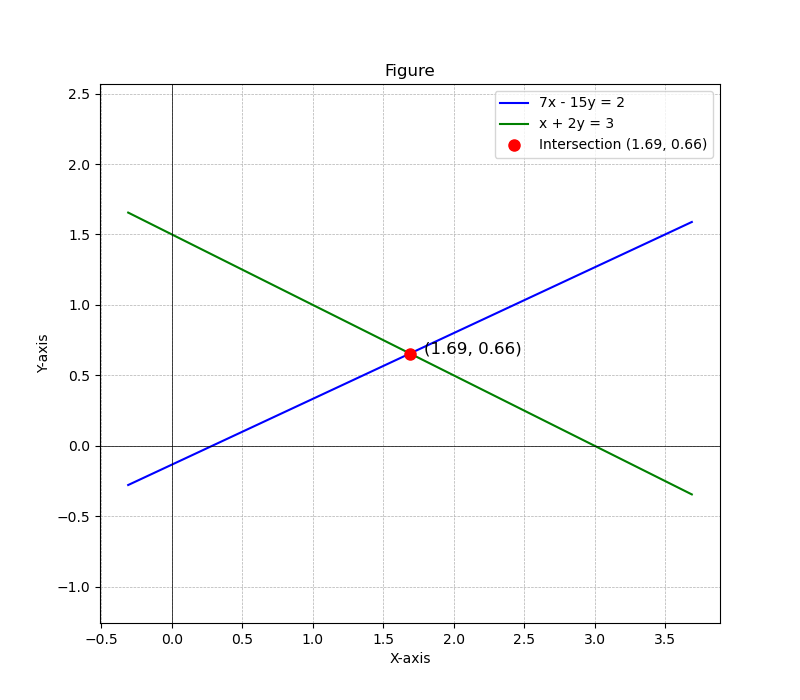
\includegraphics[width=\columnwidth, height=0.8\textheight, keepaspectratio]{figs/figure1.png}
    \end{center}
\end{frame}

\end{document}